% Definition der Klasse des Dokumentes
\documentclass[12pt, a4paper]{article}

% Standardpakete für deutsche Sprache
\usepackage[utf8]{inputenc}
\usepackage[ngerman]{babel}

\usepackage{csquotes}

% Volle Seite nutzen
\usepackage{fullpage} 
\headsep 1cm
\parindent 0cm

\usepackage{float}

% einige Pakete für Mathematische Darstellung
\usepackage{amssymb, amstext, amsmath}
\usepackage{fancyhdr}

\usepackage{booktabs}

\usepackage{listings}

% ein Paket für die Zählung von Seiten
\usepackage{count1to}
\usepackage{lastpage} 

%Paket für Aufzählungsbuchstaben
\usepackage{enumitem}

\usepackage{gensymb}

\usepackage{setspace}
\makeatletter
\newcommand{\MSonehalfspacing}{%
	\setstretch{1.44}%  default
	\ifcase \@ptsize \relax % 10pt
	\setstretch {1.448}%
	\or % 11pt
	\setstretch {1.399}%
	\or % 12pt
	\setstretch {1.433}%
	\fi
}
\newcommand{\MSdoublespacing}{%
	\setstretch {1.92}%  default
	\ifcase \@ptsize \relax % 10pt
	\setstretch {1.936}%
	\or % 11pt
	\setstretch {1.866}%
	\or % 12pt
	\setstretch {1.902}%
	\fi
}
\makeatother
\MSonehalfspacing

%\usepackage{csquotes}

% Kopfzeile und Fußzeile
\lhead{Laserprojekt}
\chead{}
\rhead{\today}
\lfoot{Jan Pohlmeyer \& Janneke Simmering}
\rfoot{\thepage\ von \pageref{LastPage}}
\cfoot{}

% Wird zur Einbindung von Bildern benötigt
\usepackage{graphicx}
\graphicspath{{pictures/}}
% Einbinden des Literaturverzeichnisses
%\usepackage[backend=bibtex,style=numeric-comp]{biblatex}
%\bibliography{literatur.bib}
%\addbibresource{literatur.bib}

% Wird zum Einbinden von LaTeX Code benötigt
\usepackage{color}
\usepackage{showexpl}

\renewcommand{\footrulewidth}{0.4pt}
\pagestyle{fancy}

% Konfiguration des Deckblatts
\begin{titlepage}
\title{\textbf{Angewandte Robotik \\ Laserprojekt}}
\author{Jan Pohlmeyer \& Janneke Simmering}
\date{\today}
\end{titlepage}

\begin{document}
% Einfügen des Deckblatts
\clearpage
\maketitle
\thispagestyle{empty}


\tableofcontents

\newpage

\section{Hindernisvermeidung (Jan)}

Damit ein mobiler Roboter eine Karte von einem Raum aufnehmen kann muss er sich natürlich durch den Raum bewegen können um alle Ecken zu erreichen. Dabei ist es unumgänglich eine Strategie zu implementieren mithilfe derer der Roboter durch den Raum fährt ohne mit Hindernissen und Wänden zu kollidieren.
Da der Laserscanner eine Reichweite von etwa 8 Metern hat muss der Raum nicht unbedingt systematisch abgefahren werden. Es reicht, wenn der Roboter alle Ecken des Raumes mit dem Laserscanner mindestens einmal aufnehmen kann.

Die Strategie, die wir zuerst implementiert haben, hat versucht leicht vom nächsten Hindernis weg zu lenken. Es wird der Scanpunkt mit dem minimalen Abstand bestimmt und wenn dieser eher auf der rechten Seite des Roboters liegt wird leicht nach links gesteuert, bzw. falls das nächste Hindernis sich eher links befindet, wird leicht rechts gesteuert. Wenn der minimale Abstand aber über einem Threshold von 1,2 Metern liegt, fährt der Roboter einfach weiter geradeaus.
Ein Problem mit diesem Ansatz trat auf, falls der Roboter in eine Sackgasse gefahren war und dann schräg vor einer der Ecken stand.
Dies haben wir zunächst versucht durch eine Sackgassenerkennung zu beheben, die auf ein lokales Maximum geradeaus vor dem Roboter prüft.
Leider hat dieser Lösungsansatz nicht so gut geklappt und häufig wurde der Autostop des Roboters ausgelöst. Da wir ein weiteres Problem dieses Ansatzes mit Löchern in den Wänden (zwischen den Kartons) sahen, haben wir uns dann entschieden den Ansatz zu wechseln.

Der neue Ansatz soll nun zum Einen das Problem der Sackgassen lösen und auch mit Spalten zwischen den Wänden klarkommen. Dazu werden die Scanpunkte zunächst in 3 gleich große Bereiche aufgeteilt. Der erste Bereich sind die Punkte, die eher zur rechten Seite des Roboters liegen. Der zweite Bereich sind die Punkte, die geradeaus vor dem Roboter liegen und der dritte Bereich sind schließlich die Punkte, die links vom Roboter liegen. In jedem der Bereiche werden nun die Scanpunkte gezählt, die einen bestimmten Distanzthreshold unterschreiten. Zunächst haben wir den Threshold auf 1,2m gesetzt, damit wir mit aktivem Autostop testen konnten.
Auch für die Anzahl Scanpunkte, ab dem ein Bereich als ''nah'' gilt wurde ein Threshold auf 5 Stück festgelegt. Dies verhindert, dass durch Ausreißerpunkte eine Hindernisvermeidung angestoßen wird und schlägt trotzdem direkt an, falls ein echtes Hindernis im Weg auftauchen sollte.
Falls sich im vorderen Bereich nun weniger Scanpunkte finden als dieser Threshold, dann wird einfach weiter der alte Ansatz verfolgt. Wenn sich allerdings im vorderen Bereich ein Hindernis befindet, dann verhält der Roboter sich anders. Zunächst vergleicht er die Anzahl Scanpunkte auf der linken und der rechten Seite deren Distanz unter dem Threshold ist. Falls links weniger Punkte als rechts sind fährt er eine scharfe links Kurve, falls rechts weniger Punkte sind eine scharfe rechts Kurve. Falls aber auf beiden Seiten ungefähr gleich viele Punkte sind und die Punkteanzahl den Threshold von 5 Punkten überschreitet geht er von einer Sackgasse aus und versucht sich umzudrehen indem er auf der Stelle dreht. Falls auf beiden Seiten ungefähr gleich viel Platz scheint fährt er einfach eine scharfe rechts Kurve.
Dieser Ansatz funktioniert ziemlich gut und wir konnten den Autostop deaktivieren um zu testen wie weit wir den Distanzthreshold verringern können. Letztendlich haben wir den Threshold auf 0,7 Meter runtergesetzt. Der Roboter vermeidet Hindernisse nun sehr zuverlässig ohne aber Ecken eines Raumes komplett auszulassen. Er schafft es sogar selbstständig durch die Labortür auf den Flur.

\section{Winkelhistogramme (Janneke)}

erster naiver ansatz (ohne rauschen)

berechne winkel der geraden wenn man einen scanpunkt mit dem nächsten verbindet (angle=atan2(y1-y2,x1-x2))
umrechnen in grad
einteilen in bins im histogramm (angle+180)/(360/BINCOUNT)
zählen in den entsprechenden bins

darstellen im histogramm fenster mit kreisen

(winkelhistogramLaserOhneRauschen)

\section{Korrelation der Winkelhistogramme}

berechnen der korrelation zwischen dem aktuellen winkelhistogramm und dem vorherigen winkelhistogram

korrelationsformel: blub

einteilen der korrlationswerte in bins

skalieren der grafischen ausgabe

\section{Rotationskorrektur (Janneke)}

Nach dem wir im letzten Kapitel die relative Rotation der Scans berechnet haben wollen wir nun den aktuellen Scan so rotieren, dass er in die Karte mit der richtigen Rotation eingetragen werden kann. Da sich der Roboter bei der Exploration nicht nur im Kreis dreht sondern auch fährt ist das Korrelationsmaximum nicht unbedingt eindeutig. Daher wird die Odometrie verwendet um das richtige Korrelationsmaximum zu finden. Um Fehler auszuschließen haben wir daher zunächst nur die Rotation die wir aus der Odometrie erhalten haben verwendet und den Scan anhand dessen rotiert. Dies hat jedoch nur beim ersten Schritt funktioniert, da wir nicht bedacht haben, dass dir so berechnete Rotation nur zum letzten Scan ist, welcher aber ja bzgl. des davor auch schon rotiert sein kann. Wir mussten also diese relative Rotation in eine globale Rotation bzgl. des ersten Scans umrechnen. Dies haben wir gelöst indem wir einen globalen Offset gespeichert haben der dann um die relative Rotation verändert wurde.

Nachdem wir jetzt sichergestellt hatten, dass es keine Fehler in anderen Teilen der Implementierung mehr gab haben wir ausgehend von der Odometrieschätzung ein lokales Maximum in der Korrelation gesucht. Unser erste Ansatz war es solange nach rechts und links um die Odometrieschätzung zu suchen, bis wir einen Wert gefunden haben, der einen bestimmten Threshold abhängig vom globalen Maximum der Korrelation übersteigt. Zunächst war dieser Threshold 50\% des maximalen Korrelationswerts, später haben wir ihn auf 75\% hochgesetzt. Dies führte jedoch zu Problemen da teilweise nicht das richtige Maximum gefunden wurde. Es wurde schnell klar, dass es gerade auf dem echten Roboter mit verrauschten Daten sehr schwer sein würde den Threshold gut einzustellen. Daher haben wir uns entschlossen stattdessen einen lokales Maximum in einem bestimmten Suchbereich um die Odometrieschätzung zu suchen. Die Größe des Suchbereichs haben wir zunächst auf 15 Grad in beide Richtungen um die Odometrieschätzung gewählt. Als Parameter lässt sich diese wesentlich einfacher optimieren und ist weniger fehleranfällig als der vorherige Ansatz, wodurch unsere Implementation wesentlich stabiler wurde.

Der Scan wird nun entsprechend des Bins des lokalen Maximum der Korrelation plus globalen Offset rotiert und in die Karte eingetragen. In der Simulation mit einem Roboter der sich nur auf der Stelle rotiert erhalten wir gute Ergebnisse.

%TODO: Bild

\section{Ausrichten der Wände auf die Hauptachsen (Janneke)}

Bisher haben wir die Translation der Karte um andere Bewegungen des Roboters auszugleichen noch gar nicht beachtet. Hierfür können X- und Y-Histogramme verwendet werden. Um ein X- bzw. Y-Histogramm zu erstellen muss allerdings der Scan hauptachsenaligned sein. D.h. das die Wände bzw. geraden Linien im Scan auf der X- bzw Y-Achse liegen muss.

Dies könnte man nur für die Erstellung der Histogramme in jedem Schritt für jeden Scan einzeln machen, wir haben uns jedoch dafür entschieden unseren initialen Scan so auszurichten da dann jeder weitere Scan durch die Rotationskorrektur auf den ersten Scan ausgerichtet wird und damit automatisch auch auf die Hauptachsen ausgerichtet wird.

Also suchen wir das Maximum im Winkelhistogramm des ersten Scans welches der prominentesten Wand entsprechen würde. Dann rotieren wir den Scan so, dass der berechnete Winkel auf die Null im Histogramm verschoben wird. Diese Rotation setzen wir dann als initialen Rotationsoffset. Der rotierte Scan wird dann in die Karte eingezeichnet, sodass unsere resultierende Karte auch direkt Hauptachsenaligned ist.

\begin{figure}
	\centering
	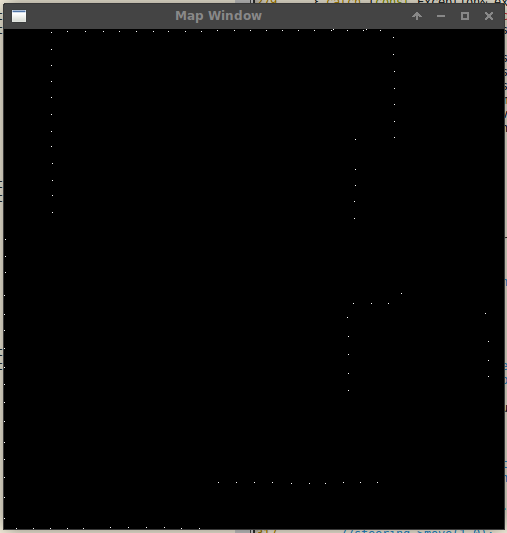
\includegraphics[width=11cm]{hauptachsenalignedMap}
	\caption{Auf die Hauptachsen ausgerichtete Karte}
	\label{fig:Hauptachsenaligned}
\end{figure}

Abbildung~\ref{fig:Hauptachsenaligned} zeigt die Karte in die der initiale auf die Hautachsen ausgerichteten Scan eingezeichnet ist.

\section{X/Y Histogramme}

auf dem achsenalignten scan werden die scan punkte in ein x und ein y histogram eingetragen

die größe der histogramme wird dabei an der maximalen laserdistanz ausgerichtet damit alle werte eingetragen werden können

\section{Korrelation der x/y Histogramme (Jan)}

erster ansatz: übertragen der lösung für die korrelation für die winkelhistogramme auf die x/y histogramme mit derselben formel

\begin{figure}
	\centering
	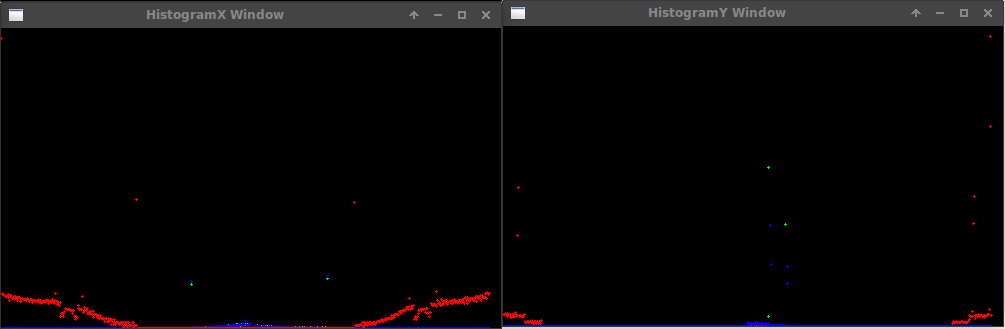
\includegraphics[width=16cm]{XYhistogram}
	\caption{X- und Y-Histogramm einer Bewegung in Y-Richtung auf eine Wand zu.}
	\label{fig:xyhistogram}
\end{figure}

\section{Translationskorrektur}

erster ansatz: berechnen des lokalen maximums der korrelation ausgehen von dem odometrie wert als mittelpunkt -> does not really work right now...

(Translation)

\subsection{Parameteroptimierung}

Da sich nun keine implementationstechnischen Fehler mehr im Programm befinden, können wir dazu übergehen die unterschiedlichen Parameter so anzupassen, dass die Karte eines durch Pappkartons errichteten Bereiches im Labor optimal aufgenommen wird.

\subsubsection{Optimierung des COUNT-Parameters (Jan)}

Der COUNT-Parameter legt fest bei welchen Schleifendurchläufen zusätzlich zur Hindernisvermeidung auch ein Karten-Update durchgeführt wird. Dies ist zum einen notwendig, damit der Roboter mit den Scans hinterherkommt und zum anderen sinnvoll, da der Roboter dann bereits eine bedeutendere Bewegung durchgeführt hat, sodass in der Differenz der Scans die Bewegungsänderung signifikanter als das Rauschen ist. Wir haben zusätzlich einen kurzen Sleep von 100ms in die Hauptschleife eingefügt, damit der Roboter mit den Scans nicht in Verzug gerät, aber trotzdem zeitnah auf auftauchende Hindernisse reagieren kann.
Wir haben den COUNT-Parameter im Bereich von 2 bis 8 getestet. Die besten Ergebnisse bekamen wir bei einem COUNT von 4, was bedeutet, dass in jedem 4. Schritt ein Karten-Update durchgeführt wird.

%TODO bilder?

\section{Aktualisieren des Referenzscans}

\subsubsection{Auflösung der Histogramme (Jan)}

Ein weiterer wichtiger Parameter ist die Auflösung der Histogramme.
Für das Winkelhistogramm ist natürlich wichtig, dass eine Rotation möglichst genau abgebildet werden kann. Falls ein Maximum sich aber auf mehrere Bins aufteilt, kann es sein, dass das Maximum nicht gefunden wird. Hier ist es deshalb wichtig einen guten Mittelweg zu finden. Initial haben wir für die Winkelhistogramme eine Binanzahl von 300 gewählt, was einer Auflösung von 1,2 Grad pro Bin entspricht. Im weiteren Verlauf haben wir die Binanzahl auf 400 erhöht, was eine leichte Verbesserung mit sich brachte. Eine Erhöhung der Binanzahl auf 500 hatte wiederum eine Verschlechterung zur Folge. Mit einer Anzahl von 550 Bins für das Winkelhistogramm haben wir letztendlich die besten Ergebnisse erzielen können. Dies entspricht einer Auflösung von etwa 0,65 Grad pro Bin.

\begin{figure}
	\centering
	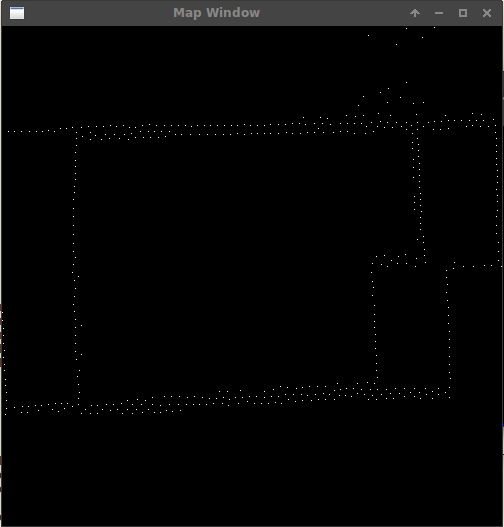
\includegraphics[width=10cm]{netzwerk}
	\caption{Verrutschen der Karte, vermutlich verursacht durch eine Netzwerkverzögerung}
	\label{fig:netzwerk}
\end{figure}

Die Anzahl der Bins für die X- und Y-Histogramme muss zusätzlich auch immer noch auf die Distanzen in der Umgebung angepasst werden. Die optimalen Ergebnisse auf dem Roboter im Testbereich im Labor erzielten wir mit 500 Bins und einer maximalen Distanz von 6 Metern. Dies entspricht einer Auflösung von 1,2 cm pro Bin.

\subsubsection{Verrutschen der Karte (Jan)}

Ab und zu kam es zu einem verrutschen der Karte. Wir nehmen an, dass hier durch eine Verzögerung des Netzwerks ein Scan zum falschen Zeitpunkt eingezeichnet wurde. Dieses Problem trat allerdings sehr selten auf und konnte auch an keinem weiteren Faktor festgemacht werden. Wie in Abbildung~\ref{fig:netzwerk} zu sehen ist, ist dadurch natürlich die Karte ungültig und es muss ein neuer Versuch gestartet werden.


\end{document}